\documentclass[unknownkeysallowed]{beamer}

\usepackage[utf8]{inputenc}
\usepackage{lmodern}

\setcounter{tocdepth}{2}

\usepackage{listings}

\usepackage{graphicx}
\usepackage{xcolor}
\usepackage{tikz}
\usetikzlibrary{arrows, snakes, backgrounds}
\usepackage{wrapfig}

% for \uptau
\usepackage{upgreek}

\title{Rate Monotonic vs. EDF: Judgment Day}
\subtitle{von Buttazzo, G. C.}
\date{\today}
\author{Dominik Schlecht}
\institute[THI]{Technische Hochschule Ingolstadt}

\usetheme{Copenhagen}

% Fix ToC-Spacing
\usepackage{etoolbox}

\makeatletter
\patchcmd{\beamer@sectionintoc}{\vskip1.5em}{\vskip0.5em}{}{}
\makeatother

\AtBeginSubsection[]
%\AtBeginSection[]
{
	\begin{frame}<beamer>
		\frametitle{Gliederung}
		\tableofcontents[
  			currentsection,
  			sectionstyle=show/show,
  			subsectionstyle=show/shaded/hide,
  			squeeze
		]
	\end{frame}
}

\begin{document}
	\frame{\maketitle}
	\frame{\tableofcontents[hideallsubsections]}
	
	
	\section{Einleitung}
	\subsection{Meta-Informationen}
\begin{frame}{\subsecname}
	\begin{itemize}
		\item Author:
		\begin{itemize}
			\item Giorgio C. Buttazzo
			\item University of Pavia, Italien
			\item buttazzo@unipv.it
		\end{itemize}
		\item Whitepaper
		\begin{itemize}
			\item Rate Monotonic vs. EDF: Judgment Day
			\item Real-Time Systems, 29, 5–26, 2005
		\end{itemize}						
		
	\end{itemize}
\end{frame} 

\subsection{Abstract}
\begin{frame}{\subsecname}
\tiny Since the first results published in 1973 by Liu and Layland on the Rate Monotonic (RM) and Earliest Deadline First (EDF) algorithms, a lot of progress has been made in the schedulability analysis of periodic task sets. Unfortunately, many misconceptions still exist about the properties of these two scheduling methods, which usually tend to favor RM more than EDF. Typical wrong statements often heard in technical conferences and even in research papers claim that RM is easier to analyze than EDF, it introduces less runtime overhead, it is more predictable in overload conditions, and causes less jitter in task execution.Since the above statements are either wrong, or not precise \tiny, it is time to clarify these issues in a systematic fashion, because the use of EDF allows a better exploitation of the available resources and significantly improves system’s performance. This paper compares RM against EDF under several aspects, using existing theoretical results, specific simulation experiments, or simple counterexamples to show that many common beliefs are either false or only restricted to specific situations.\footnote{Rate Monotonics vs. EDF: Judgment Day, Girorgio C. Buttazzo, 2005}
\end{frame}

\begin{frame}{\subsecname}
\includegraphics[width=\textwidth]{graphics/memes/aintnobody.jpg}
\end{frame}

\begin{frame}{\subsecname}
\tiny Since the first results published in 1973 by Liu and Layland on the Rate Monotonic (RM) and Earliest Deadline First (EDF) algorithms, a lot of progress has been made in the schedulability analysis of periodic task sets. Unfortunately, many \Large misconceptions \tiny still exist about the properties of these two scheduling methods, which usually tend to favor RM more than EDF. Typical wrong statements often heard in technical conferences and even in research papers claim that RM is easier to analyze than EDF, it introduces less runtime overhead, it is more predictable in overload conditions, and causes less jitter in task execution.Since the above statements are either wrong, or not precise, it is time to clarify these issues in a systematic fashion, because the use of EDF allows a better exploitation of the available resources and significantly improves system’s performance. This paper compares RM against EDF under several aspects, using existing theoretical results, specific simulation experiments, or simple counterexamples to show that many common beliefs are either false or only restricted to specific situations.\footnote{Rate Monotonics vs. EDF: Judgment Day, Girorgio C. Buttazzo, 2005}
\end{frame}
	
\begin{frame}{\subsecname}
\tiny Since the first results published in 1973 by Liu and Layland on the Rate Monotonic (RM) and Earliest Deadline First (EDF) algorithms, a lot of progress has been made in the schedulability analysis of periodic task sets. Unfortunately, many \Large misconceptions \tiny still exist about the properties of these two scheduling methods, which usually tend to \Large favor RM more than EDF \tiny. Typical wrong statements often heard in technical conferences and even in research papers claim that RM is easier to analyze than EDF, it introduces less runtime overhead, it is more predictable in overload conditions, and causes less jitter in task execution.Since the above statements are either wrong, or not precise, it is time to clarify these issues in a systematic fashion, because the use of EDF allows a better exploitation of the available resources and significantly improves system’s performance. This paper compares RM against EDF under several aspects, using existing theoretical results, specific simulation experiments, or simple counterexamples to show that many common beliefs are either false or only restricted to specific situations.\footnote{Rate Monotonics vs. EDF: Judgment Day, Girorgio C. Buttazzo, 2005}
\end{frame}

	\begin{frame}{\subsecname}
\tiny Since the first results published in 1973 by Liu and Layland on the Rate Monotonic (RM) and Earliest Deadline First (EDF) algorithms, a lot of progress has been made in the schedulability analysis of periodic task sets. Unfortunately, many \Large misconceptions \tiny still exist about the properties of these two scheduling methods, which usually tend to \Large favor RM more than EDF \tiny. Typical wrong statements often heard in technical conferences and even in research papers claim that RM is easier to analyze than EDF, it introduces less runtime overhead, it is more predictable in overload conditions, and causes less jitter in task execution.Since the above statements are \Large  either wrong, or not precise \tiny, it is time to clarify these issues in a systematic fashion, because the use of EDF allows a better exploitation of the available resources and significantly improves system’s performance. This paper compares RM against EDF under several aspects, using existing theoretical results, specific simulation experiments, or simple counterexamples to show that many common beliefs are either false or only restricted to specific situations.\footnote{Rate Monotonics vs. EDF: Judgment Day, Girorgio C. Buttazzo, 2005}
\end{frame}
	
\begin{frame}{\subsecname}
\tiny Since the first results published in 1973 by Liu and Layland on the Rate Monotonic (RM) and Earliest Deadline First (EDF) algorithms, a lot of progress has been made in the schedulability analysis of periodic task sets. Unfortunately, many \Large misconceptions \tiny still exist about the properties of these two scheduling methods, which usually tend to \Large favor RM more than EDF \tiny. Typical wrong statements often heard in technical conferences and even in research papers claim that RM is easier to analyze than EDF, it introduces less runtime overhead, it is more predictable in overload conditions, and causes less jitter in task execution.Since the above statements are \Large  either wrong, or not precise \tiny, it is time to clarify these issues in a systematic fashion, because the use of EDF allows a better exploitation of the available resources and significantly improves system’s performance. \Large This paper compares RM against EDF \tiny under several aspects, using existing theoretical results, specific simulation experiments, or simple counterexamples to show that many common beliefs are either false or only restricted to specific situations.\footnote{Rate Monotonics vs. EDF: Judgment Day, Girorgio C. Buttazzo, 2005}
\end{frame}


\begin{frame}{\subsecname}
	\begin{center}
		\includegraphics[scale=0.6]{graphics/memes/mythbusters_thisweek.jpg}
	\end{center}
\end{frame}

%\section{Erläuterung}
\subsection{Flashback - Scheduling}
\begin{frame}{\subsecname}
	Wir definieren:
	\begin{equation}
		\uptau_{i, k} \text{ als Job mit einer absoluten Deadline } d_{i, k}
	\end{equation}
	\pause
	\begin{equation}
		\uptau_i \text{ als infinite Folge von Jobs } \uptau_{i, k} \text{ mit }
	\end{equation}
	\pause
	\begin{equation}
		\begin{array}{l l l}
			\text{Wort-Case-Execution-Time } & C_i\\
			\text{Task-Period } & T_i
		\end{array}
	\end{equation}
\end{frame}

\begin{frame}
	Klartext:\\
	\begin{center}
		%\rowcolors{1}{RoyalBlue!20}{RoyalBlue!5}
		\begin{tabular}{c||c|c}
			Task ($\uptau_i$) & Dauer ($C_i$) & Task-Periode ($T_i$)\\\hline\hline
			$\uptau_i$ & 5 & 15
		\end{tabular}
	\end{center}
\end{frame}

\begin{frame}
	\input{graphics/einleitung/simple1.tex}
\end{frame}

\begin{frame}
	\begin{figure}[htbp]
	% Partly taken from http://www.texample.net/tikz/examples/convolution-of-two-functions/
	\centering
	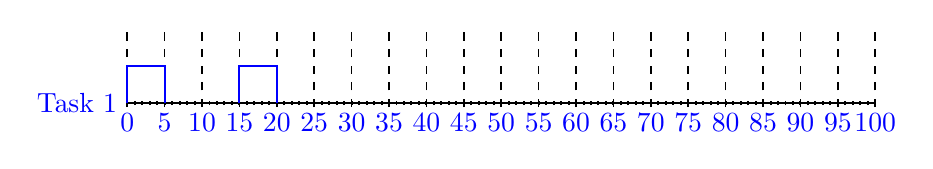
\begin{tikzpicture}[
		scale=0.095,
		line width=0.25mm,
		every node/.style={scale=1, text=blue},
		major tick/.style={semithick, dashed},
		x tick label/.style={anchor=north, minimum width=5mm},
		task1/.style={blue},
		task2/.style={red},
		task3/.style={green},
		desc/.style={anchor=east}
		]
	
	% Task 1
	\draw (0, 0) -- (100, 0);
	\node[desc] at (0, 0) {Task 1};
	
%	% Task 2
%	\draw (0, 10) -- (100, 10);
%	\node[desc] at (0, 10) {Task 2};	
%	
%	% Task 3
%	\draw (0, 20) -- (100, 20);
%	\node[desc] at (0, 20) {Task 3};	
	
	% Small ticks
	\foreach \x in {0, 1,...,100}{
		\draw (\x, -0.25) -- (\x, 0.25);
	}
	
	% Major ticks with label
	\foreach \x/\label in {0, 5,...,100}{
		\node[x tick label] at (\x, 0) {$\label$}; 		
		\draw[major tick] (\x, -0.5) -- (\x, 10);
	}
	
	% Draw all
%	\foreach \x in {0, 15,...,100}{
%		\draw[task1] (\x, 0) -- (\x, 5) -- (\x+5, 5) -- (\x+5, 0);
%	}
	
	% Single steps for the slides
	\draw[task1] (0, 0) -- (0, 5) -- (5, 5) -- (5, 0);
	\draw[task1] (15, 0) -- (15, 5) -- (20, 5) -- (20, 0);
%	\draw[task1] (30, 0) -- (30, 5) -- (35, 5) -- (35, 0);
%	\draw[task1] (45, 0) -- (45, 5) -- (50, 5) -- (50, 0);
%	\draw[task1] (60, 0) -- (60, 5) -- (65, 5) -- (65, 0);
%	\draw[task1] (75, 0) -- (75, 5) -- (80, 5) -- (80, 0);
%	\draw[task1] (90, 0) -- (90, 5) -- (95, 5) -- (95, 0);

	\end{tikzpicture}
\end{figure}
\end{frame}

\begin{frame}
	\begin{figure}[htbp]
	% Partly taken from http://www.texample.net/tikz/examples/convolution-of-two-functions/
	\centering
	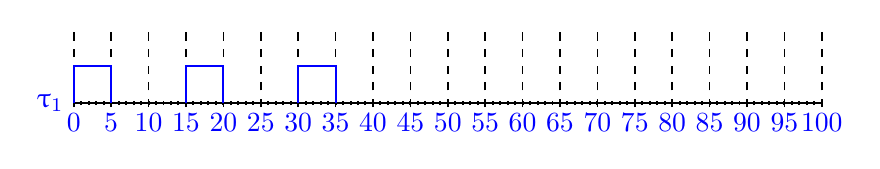
\begin{tikzpicture}[
		scale=0.095,
		line width=0.25mm,
		every node/.style={scale=1, text=blue},
		major tick/.style={semithick, dashed},
		x tick label/.style={anchor=north, minimum width=5mm},
		task1/.style={blue},
		task2/.style={red},
		task3/.style={green},
		desc/.style={anchor=east}
		]
	
	% Task 1
	\draw (0, 0) -- (100, 0);
	\node[desc] at (0, 0) {$\uptau_1$};
	
	\foreach \x in {0, 1,...,100}{
		\draw (\x, -0.25) -- (\x, 0.25);
	}
	
	% Major ticks with label
	\foreach \x/\label in {0, 5,...,100}{
		\node[x tick label] at (\x, 0) {$\label$}; 		
		\draw[major tick] (\x, -0.5) -- (\x, 10);
	}
	
	
	% Single steps for the slides
	\draw[task1] (0, 0) -- (0, 5) -- (5, 5) -- (5, 0);
	\draw[task1] (15, 0) -- (15, 5) -- (20, 5) -- (20, 0);
	\draw[task1] (30, 0) -- (30, 5) -- (35, 5) -- (35, 0);

	\end{tikzpicture}
\end{figure}
\end{frame}

\begin{frame}
	\input{graphics/einleitung/simple4.tex}
\end{frame}

\begin{frame}
	2 Tasks:
	\begin{center}
		\begin{tabular}{c||c|c}
				Task ($\uptau_i$) & Dauer ($C_i$) & Task-Periode ($T_i$)\\\hline\hline
				$\uptau_1$ & 5 & 15\\
				$\uptau_2$ & 10 & 40\\
		\end{tabular}
	\end{center}
\end{frame}

\begin{frame}
	\begin{figure}[htbp]
	% Partly taken from http://www.texample.net/tikz/examples/convolution-of-two-functions/
	\centering
	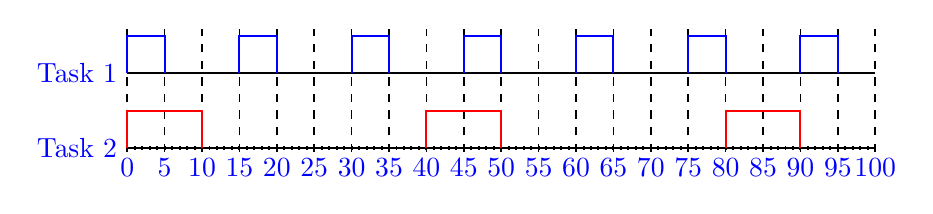
\begin{tikzpicture}[
		scale=0.095,
		line width=0.25mm,
		every node/.style={scale=1, text=blue},
		major tick/.style={semithick, dashed},
		x tick label/.style={anchor=north, minimum width=5mm},
		task1/.style={blue},
		task2/.style={red},
		task3/.style={green},
		desc/.style={anchor=east}
		]

	% Task 1
	\draw (0, 10) -- (100, 10);
	\node[desc] at (0, 10) {Task 1};
	
	% Task 2
	\draw (0, 0) -- (100, 0);
	\node[desc] at (0, 0) {Task 2};	
	
	% Small ticks
	\foreach \x in {0, 1,...,100}{
		\draw (\x, -0.25) -- (\x, 0.25);
	}
	
	% Major ticks with label
	\foreach \x/\label in {0, 5,...,100}{
		\node[x tick label] at (\x, 0) {$\label$}; 		
		\draw[major tick] (\x, -0.5) -- (\x, 16);
	}
	
	% Draw all Task 1
	\foreach \x in {0, 15,...,100}{
		\draw[task1] (\x, 10) -- (\x, 15) -- (\x+5, 15) -- (\x+5, 10);
	}
	
	% Draw all Task 2
	\foreach \x in {0, 40,...,100}{
		\draw[task2] (\x, 0) -- (\x, 5) -- (\x+10, 5) -- (\x+10, 0);
	}
	
	\end{tikzpicture}
\end{figure}
\end{frame}

\begin{frame}
	\begin{figure}[htbp]
	% Partly taken from http://www.texample.net/tikz/examples/convolution-of-two-functions/
	\centering
	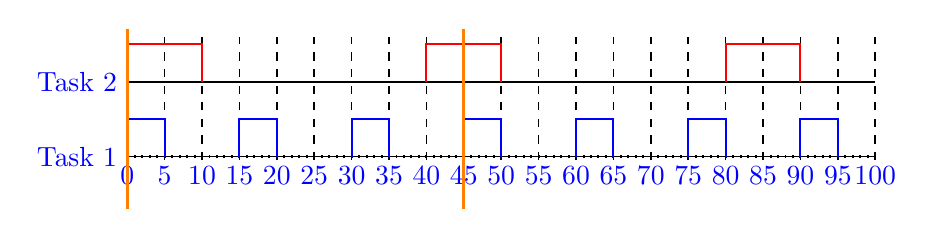
\begin{tikzpicture}[
		scale=0.095,
		line width=0.25mm,
		every node/.style={scale=1, text=blue},
		major tick/.style={semithick, dashed},
		x tick label/.style={anchor=north, minimum width=5mm},
		task1/.style={blue},
		task2/.style={red},
		task3/.style={green},
		desc/.style={anchor=east},
		konf/.style={orange, very thick}
		]
	
	% Task 1
	\draw (0, 0) -- (100, 0);
	\node[desc] at (0, 0) {Task 1};
	
	% Task 2
	\draw (0, 10) -- (100, 10);
	\node[desc] at (0, 10) {Task 2};	
%	
%	% Task 3
%	\draw (0, 20) -- (100, 20);
%	\node[desc] at (0, 20) {Task 3};	
	
	% Small ticks
	\foreach \x in {0, 1,...,100}{
		\draw (\x, -0.25) -- (\x, 0.25);
	}
	
	% Major ticks with label
	\foreach \x/\label in {0, 5,...,100}{
		\node[x tick label] at (\x, 0) {$\label$}; 		
		\draw[major tick] (\x, -0.5) -- (\x, 16);
	}
	
	% Draw all
	\foreach \x in {0, 15,...,100}{
		\draw[task1] (\x, 0) -- (\x, 5) -- (\x+5, 5) -- (\x+5, 0);
	}
	
	% Draw all
	\foreach \x in {0, 40,...,100}{
		\draw[task2] (\x, 10) -- (\x, 15) -- (\x+10, 15) -- (\x+10, 10);
	}
	
	\draw[konf] (0, 17) -- (0, -7);
	\draw[konf] (45, 17) -- (45, -7);
	
	\end{tikzpicture}
\end{figure}
\end{frame}

	
	\section{Rate Monotonic \& Erliest Deadline First}
	\subsection{Grundlagen}
\begin{frame}{\subsecname}
		\begin{columns}[]
  			\begin{column}{0.5\textwidth}
				Rate Monotonics:
				\begin{itemize}
					\item Task $T_i$ mit kürzester Periode wird bevorzugt
					\item Task $T_i$ wird anfangs eine Priorität zugewiesen
				\end{itemize}

			\end{column}
  			\begin{column}{0.5\textwidth}
  				Erliest Deadline First:
				\begin{itemize}
					\item Job $T_{i, k}$ mit der nächsten Deadline wird bevorzugt
					\item In diesem Paper ist die Deadline gleich mit der Periode
					\item Die Priorität von Task $T_i$ entscheidet sich während der Laufzeit
				\end{itemize}	
  			\end{column}
		\end{columns}
\end{frame}

\subsection{Beispiele}

\newcommand{\showRMSlide}[1] {\begin{frame}{Beispiel Rate Monotonics}
	\begin{center}
		\begin{tabular}{l||c|c}
				Task ($\uptau_i$) & Dauer ($C_i$) & Task-Periode ($T_i$)\\\hline\hline
				$\uptau_1$ & 4 & 10\\
				$\uptau_2$ & 2 & 16\\
				$\uptau_3$ & 8 & 20\\
		\end{tabular}
	\end{center}
	\input{graphics/rm/rm#1.tex}
\end{frame}}

\forloop{ct}{0}{\value{ct} < 11}%
{%
	\showRMSlide{\arabic{ct}}
}

\newcommand{\showEDFSlide}[1] {\begin{frame}{Beispiel Erliest Deadline First}
	\begin{center}
		\begin{tabular}{l||c|c}
				Task ($\uptau_i$) & Dauer ($C_i$) & Task-Periode ($T_i$)\\\hline\hline
				$\uptau_1$ & 4 & 10\\
				$\uptau_2$ & 2 & 16\\
				$\uptau_3$ & 8 & 20\\
		\end{tabular}
	\end{center}
	\input{graphics/edf/edf#1.tex}
\end{frame}}

\forloop{ct}{1}{\value{ct} < 14}%
{%
	\showEDFSlide{\arabic{ct}}
}

	%\section{Erliest Deadline First}
	%\begin{frame}{\subsecname}
		Test EDF
\end{frame}
	
	\section{Vergleich}
	\subsection{Implementation Complexity}
\begin{frame}{\subsecname}
	Frage:
	\begin{itemize}
		\item Wie groß ist der Aufwand das Scheduling-Verfahren zu implementieren?
	\end{itemize}
	Antwort:
	\begin{itemize}
		\item Rate Monotonics ist einfacher zu implementieren!
	\end{itemize}
\end{frame}

\begin{frame}{\subsecname}
	Ist es so einfach?\\\pause
	Faktoren:
	\begin{itemize}
		\item Wird auf einem bestehenden System entwickelt?
		\item Sind die Prioritäten festgesetzt oder können diese während der Laufzeit verändert werden?
		\item Wie viele Prioritäts-Level gibt es? %TODO Beispiel?
	\end{itemize}
\end{frame}

\begin{frame}{\subsecname}
	Annahme
	\begin{itemize}
		\item Das System wird von Grund auf mit einer Ready-Qeue implementiert\pause
		\item In dieser werden die Tasks für Rate Monotonics
			\begin{itemize}
				\item absteigend nach nach den Proritäten-Leveln
			\end{itemize}
			und für Erliest Deadline First
			\begin{itemize}
				\item aufsteigend nach der absoluten Deadline
			\end{itemize} gespeichert.
	\end{itemize}
\end{frame}

\subsection{Runtime Overhead}
\begin{frame}{\subsecname}
	Test
\end{frame}

\subsection{Schedulability Analysis}
\begin{frame}{\subsecname}
	Test
\end{frame}

\subsection{Robustnes During Overloads}
\begin{frame}{\subsecname}
	Test
\end{frame}

\subsubsection{Permanent Overload}
\begin{frame}{\subsecname}
	Test
\end{frame}

\subsubsection{Transient Overload}
\begin{frame}{\subsecname}
	Test
\end{frame}

\subsection{Jitter and Latency}
\begin{frame}{\subsecname}
	Test
\end{frame}

\subsection{Other Issues}
\begin{frame}{\subsecname}
	Test
\end{frame}
	
	%\section{Abschluss}
	\section{Fazit}
	\begin{frame}{\secname}
	Vorteile von Rate Monotonics:
	\begin{itemize}
		\item leichtere Implementierung in kommerziellen Systemen
	\end{itemize}
	Vorteile Erliest Deadline First:
	\begin{itemize}
		\item Erlaubt volle Auslastung des Prozessors %TODO
		\item Weniger Runtime Overhead
	\end{itemize}
	Unentschieden oder Situationsabhängig:
	\begin{itemize}
		\item Overload Situations
		\item Jitter Control
	\end{itemize}
\end{frame}

\begin{frame}{\secname}
	\begin{center}
		\includegraphics[scale=0.35]{graphics/memes/success.jpg}
	\end{center}
\end{frame}
	
	\begin{frame}{\subsecname}
		Fragen?
	\end{frame}
	
\end{document}